\documentclass{article}

\usepackage[letterpaper,margin={1.5cm}]{geometry}
\usepackage{amsmath, amssymb, amsfonts}

\usepackage[utf8]{inputenc}
\usepackage[T1]{fontenc}
\usepackage[spanish]{babel}
\usepackage{graphicx,enumitem}
\usepackage{multicol}
\usepackage{hyperref}
\usepackage{pdfpages}

\title{Enseñanza de la mecánica cuántica asistida por documentos interactivos. \\ Reporte de proyecto}
\author{Semillero Física Teórica y Computacional}

\begin{document}
\maketitle

\abstract{El uso de las nuevas tecnologías en la educación permite integrar herramientas interactivas que permiten un acercamiento mas simple a la exploración de conceptos y de la interpretación de como los parámetros de un sistema afectan su comportamiento. Una manera de lograrlo se puede aproximar mediante la separación del uso de las herramientas en 3 etapas, encargadas respectivamente de la visualización e interacción, la solución numérica y la exploración del concepto físico. Para este reporte se presenta como caso de estudio la exploración de las soluciones de estados ligados 1D.}

\section{Introducción}

El uso de las herramientas computacionales a permitido transformar las metodologías de enseñanza y acercar áreas comúnmente muy teóricas y de largos desarrollos matemáticos a procesos que pueden centrarse mucho mas en el concepto físico que en la matemática requerida \cite{Rojas2009, Landau2011}. Su aprovechamiento en su fondo requiere del desarrollo de la física computacional, que constituye el desarrollo de métodos computacionales para la solución de problemas físicos \cite{Rojas2009}.

La solución completa del problema físico no constituye la sola obtención de un resultado numérico sino la adecuada representación de los mismos y su interpretación, la cual mediante visualización se puede asistir el proceso.

Alrededor de estas iniciativas, y con especial enfoque en la mecánica cuántica existen acercamientos mediante \textit{applets} \cite{Belloni2015}, aplicaciones en html5 y javascript \cite{UCB2015}, códigos con métodos simples como diferencias finitas \cite{Garcia2007} y graficación tradicional y experiencias en HUBs con NanoHUBS \cite{Klimeck2007}. Se presenta un gran uso del lenguaje python para este tipo de aplicaciones cuando son de uso local (no web) \cite{Rojas2009, Landau2011} por su sencilla sintaxis y amplio soporte.

Mas recientemente, la integración de documentos interactivos de formatos abiertos (ipython notebooks y sage notebooks) \cite{Perez2013, Shen2014} y cerrados (maple worksheets) \cite{Horbatsch1995} ha permitido llevar a un solo ambiente, continuo y natural, las simulaciones y visualizaciones con sus respectivos materiales de apoyo, con especial interés aquellos formatos libres que brindan una mayor accesibilidad.

\section{Método}

Se desarrollo una metodología de documentos interactivos usando el formato abierto de Jupyter Notebook (anteriormente IPython Notebook) con integración de elementos interactivos \textit{widgets} para la exploración de parámetros \cite{Jupyter2015}.

El documento interactivo se divide en 3 documentos acorde a la separación metodológica de la solución del problema físico, que se expone como parte de los tópicos básicos requeridos en física computacional en distintos currículos \cite{Landau2006, Landau2011}

\begin{itemize}
\item Visualización e interacción: Se exponen las necesidades de representación de los datos y la forma de realización, así como el uso de los controles para la interacción.
\item Técnicas numéricas. Se expone las técnicas de aproximación numérica y su aplicación al contexto para la búsqueda de raíces y ecuaciones diferenciales con problema de frontera, y la metodología para contribuir a la estabilidad de las soluciones mediante el rescalamiento de valores por adimensionalización de la ecuación diferencial.
\item Conceptualización física. Se presentan los elementos físicos habilitando una interacción amplia de los parámetros físicos y numéricos del fenómeno expuesto. Al respecto se explora el caso de estudio de estados ligados y superposición.
\end{itemize}

La accesibilidad del recurso es posible gracias al almacenamiento gratuito y publico ofrecido por el servidor git de \href{https://github.com/}{github}\footnote{https://github.com/}, y la ejecución en un servidor local posible mediante la instalación libre de jupyter notebooks o de su ejecución en servicios en linea gratuitos o por suscripción como \href{https://cloud.sagemath.com/}{SageMath} \footnote{https://cloud.sagemath.com/} o \href{https://www.authorea.com/}{Authorea}\footnote{https://www.authorea.com/}.

Para una mayor discusión de los tópicos de la metodología, remítase a los notebooks, cuya versión estática se anexa a este documento.

\section{Resultados}

Se genera satisfactoriamente la integración en documentos interactivos de formato abierto y gratuitos de desarrollos numéricos con estrategia de visualización e interacción de conceptos de la mecánica cuántica, con la presentación de casos de estudio de estados ligados y el concepto de paquete de onda.

La estrategia planteada permite crear un apoyo al desarrollo de un curso de mecánica cuántica sin dependencia de conocimientos previos en programación ni requerimientos específicos de instalaciones, salvo contar con un navegador web y acceso a internet. Siendo así una estrategia reproducible en otras instituciones sin limitación por requerimientos de una plataforma para la ejecución de los documentos interactivos.

Se logra independizar claramente las etapas en la estrategia de solución y así permitir el abordaje del problema físico con 3 niveles según el interés que se posea en las herramientas numéricas y de visualización, o si solo se trata del apoyo como recurso para la exploración de parámetros.

Una versión estática de los notebooks se anexa al reporte. Para su versión interactiva esta puede ser descargada del repositorio github \href{https://github.com/fisicatyc/Cuantica\_Jupyter}{Cuantica\_Jupyter}\footnote{https://github.com/fisicatyc/Cuantica\_Jupyter} del semillero\footnote{https://github.com/fisicatyc} y cargarlos en un servidor jupyter (de instalación local o de un servicio en linea como sagemath, el cual es recomendado).

Para simulaciones con tiempos de ejecución altos, el servidor notebook retira la instancia tras un cierto lapso de tiempo. Para este tipo de casos se recomienda el uso directo de ipython o python.

\section{Conclusiones}

Es posible integrar de una manera natural las etapas de solución de un problema físico sin generar un solapamiento de un elemento con otro, que afecte el proceso de aprendizaje en medio del desarrollo y lectura de códigos de visualización y simulación, al separar estos en términos de la presentación con su respectiva documentación que permita no solo interactuar el documento de apoyo del curso original sino también una interacción con los nuevos elementos que se incorporan.

Al no ser complejos los elementos nuevos, se puede usar el documento conceptual como apoyo a los currículos tradicionales sin requerir de algún conocimiento de programación. Los elementos nuevos en la metodológia, permiten un acercamiento para cursos con un enfoque en computación y visualización científica, para el cual si es requerido un conocimiento previo en programación.

Es posible aumentar la accesibilidad de este recurso a un mayor publico gracias a ser un formato y herramienta abierta y gratuita, permitiendo una fácil descarga e instalación en caso de uso local o el uso de servicios en linea (gratuitos o por suscripción) que ofrecen servidos de jupyter notebook, dependiendo solo de conectividad a internet sin requerimientos especiales de hardware.

Para potenciales no simétricos y con amplias diferencias entre el potencial máximo y mínimo se recomienda usar instancias directas de python e ipython, debido al comportamiento como servidor de las instancias de Jupyter, que provocan la terminación del llamado al kernel tras un \textit{timeout}, de aproximadamente minuto y medio. Tras este periodo se recomienda reiniciar el kernel (tanto si es de ejecución local como en linea).

\bibliographystyle{unsrt}
\bibliography{reporte}

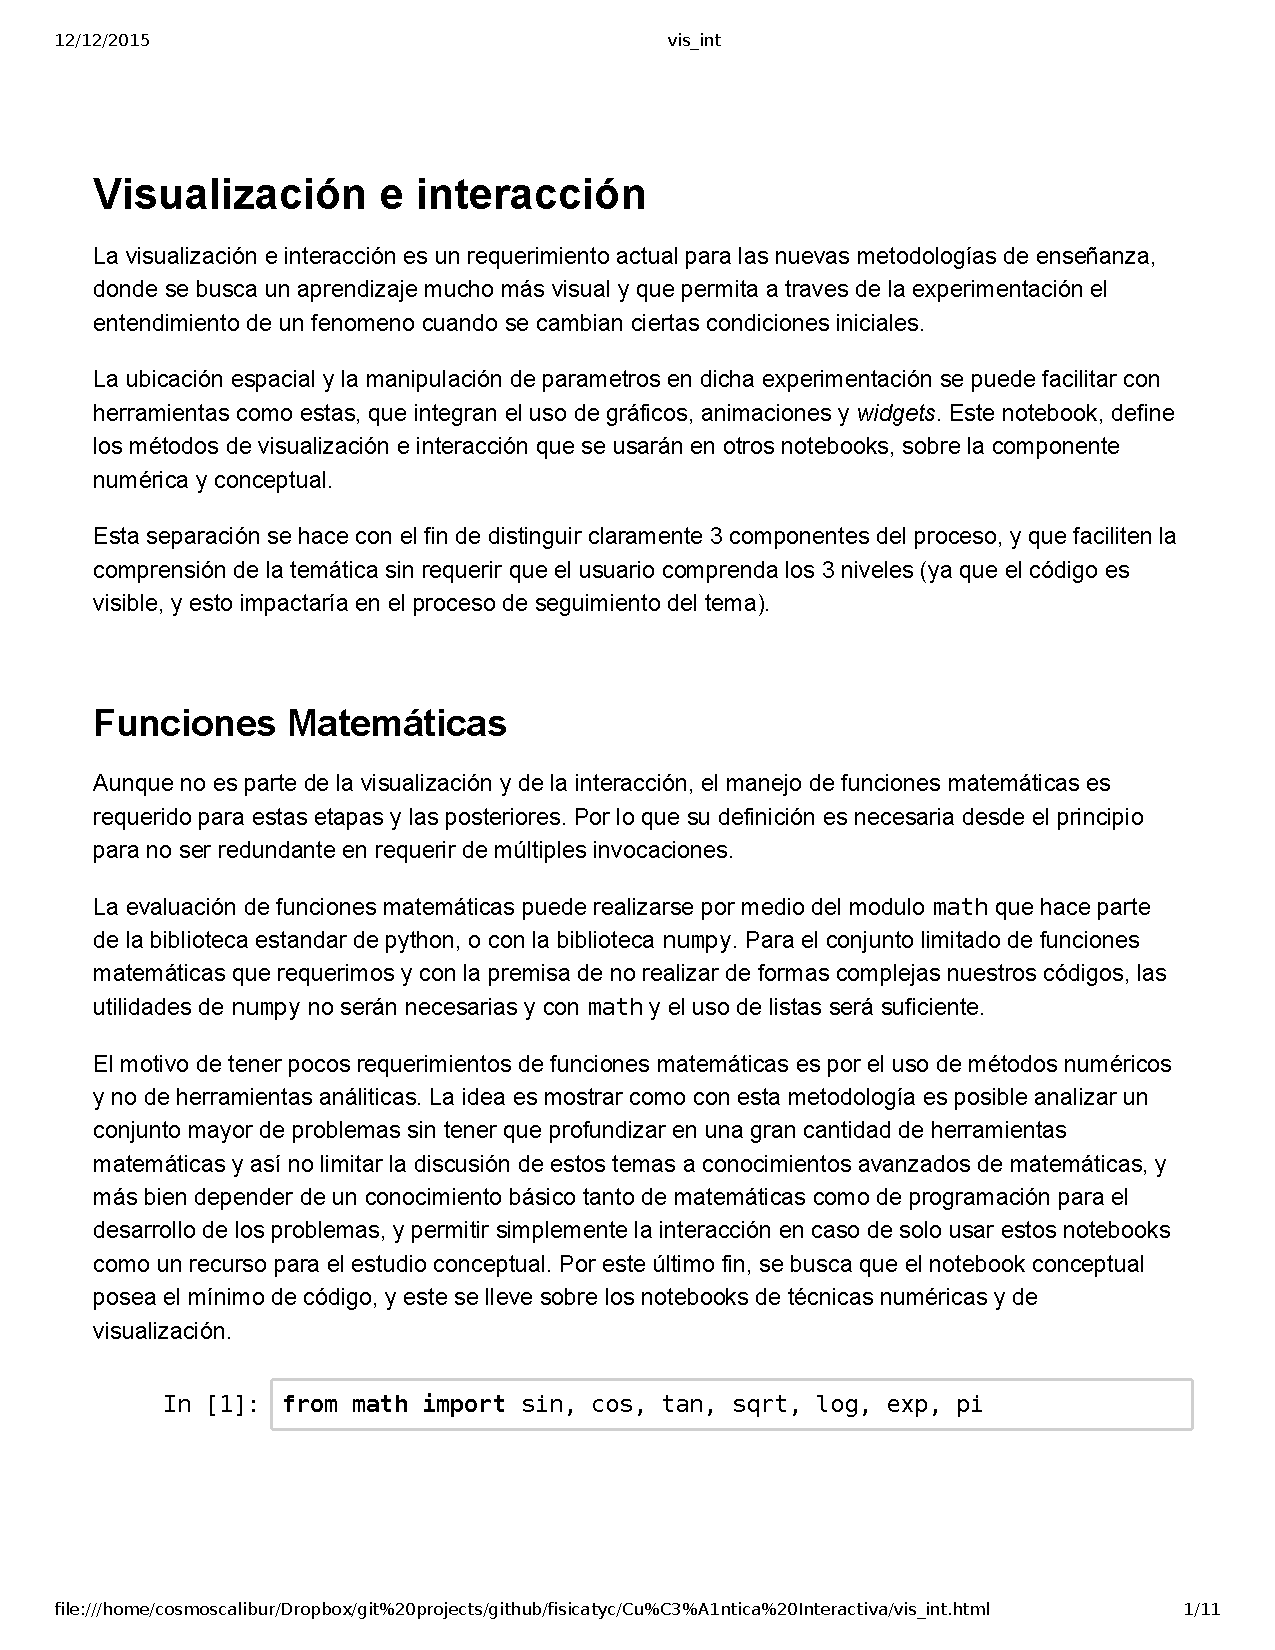
\includepdf[pages=-]{vis_int.pdf}
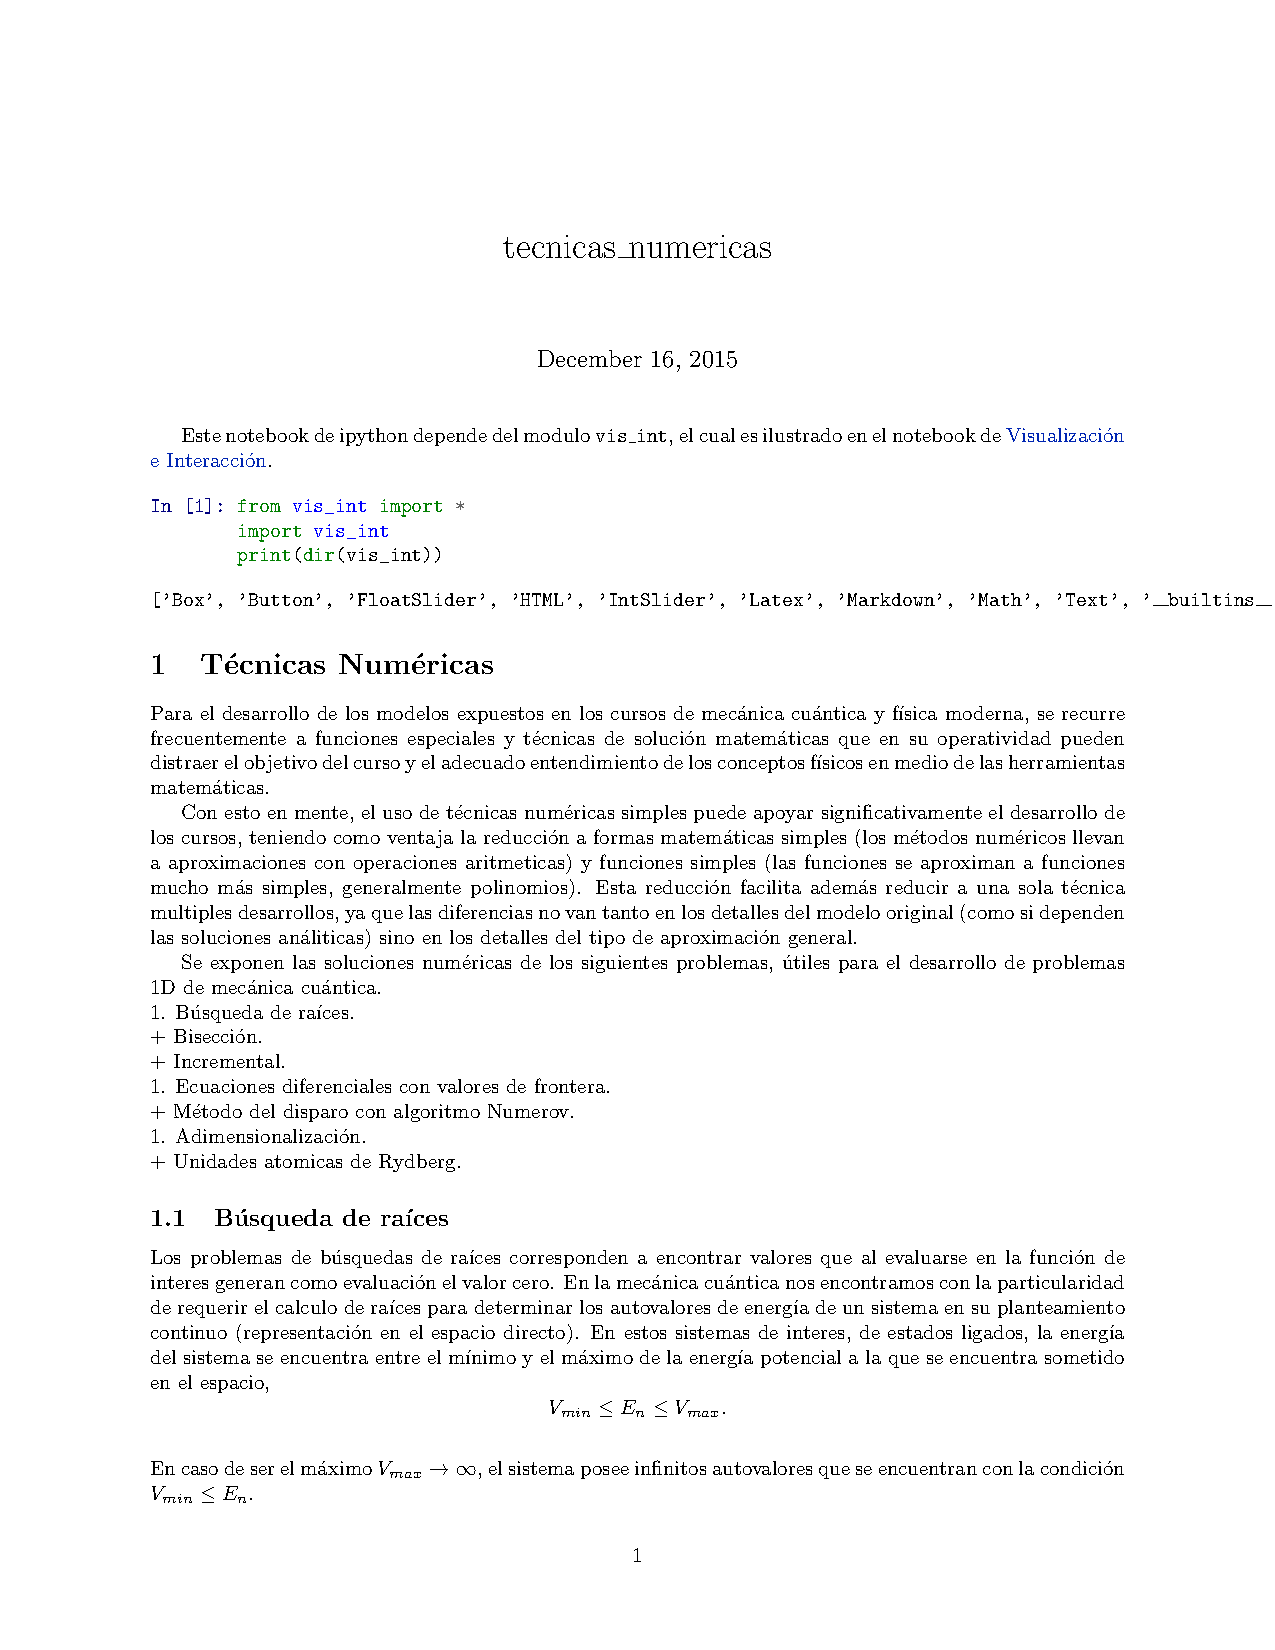
\includepdf[pages=-]{tec_num.pdf}
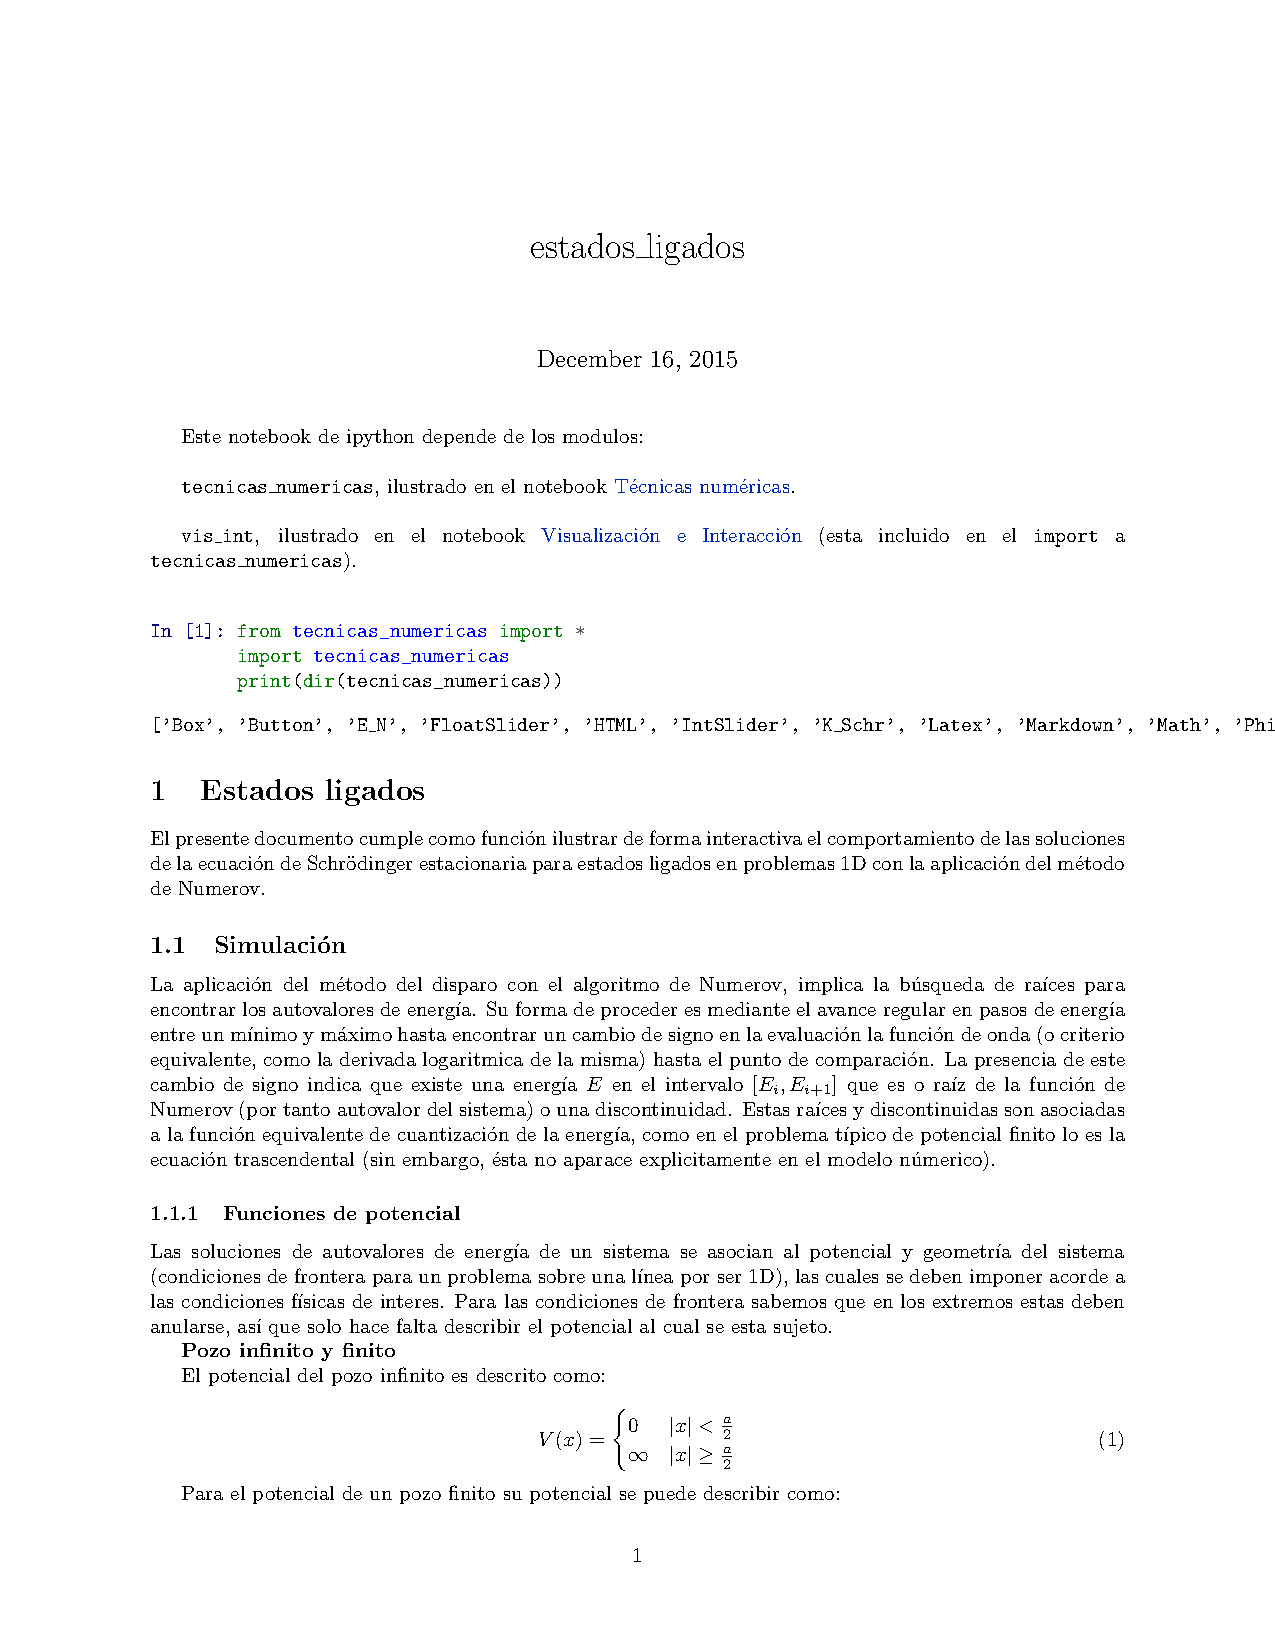
\includepdf[pages=-]{est_lig.pdf}

\end{document}
